% !TEX root = ../report.tex

\chapter{Introduction}
\label{chap:introduction}
\minitoc
\setcounter{page}{1}
\pagenumbering{arabic}
\clearpage

\newcommand{\ecommercenorway}[0]{
  \begin{figure}[H]
    \centering
    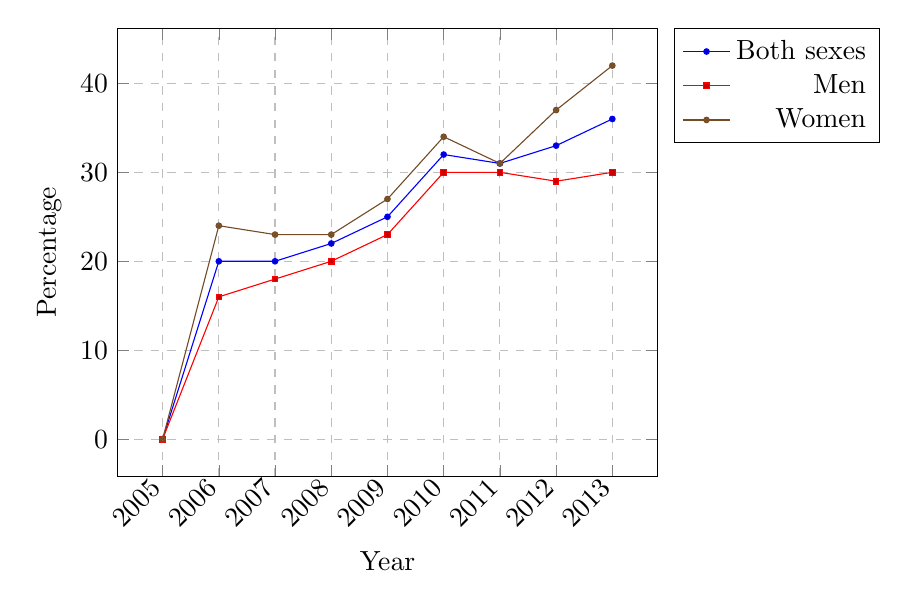
\begin{tikzpicture}
      \begin{axis}[
        xlabel={Year},
        ylabel={Percentage},
        legend style={cells={anchor=east}, legend pos=outer north east,},
        xtick=data,
        x tick label style={rotate=45, anchor=east, /pgf/number format/1000 sep=},
        mark size=1.0pt,
        grid=major,
        grid style={dashed},
      ]
      \legend{Both sexes, Men, Women}
      \addplot coordinates {
        (2005, 0)
        (2006, 20)
        (2007, 20)
        (2008, 22)
        (2009, 25)
        (2010, 32)
        (2011, 31)
        (2012, 33)
        (2013, 36)
      };
      \addplot coordinates {
        (2005, 0)
        (2006, 16)
        (2007, 18)
        (2008, 20)
        (2009, 23)
        (2010, 30)
        (2011, 30)
        (2012, 29)
        (2013, 30)
      };
      \addplot coordinates {
        (2005, 0)
        (2006, 24)
        (2007, 23)
        (2008, 23)
        (2009, 27)
        (2010, 34)
        (2011, 31)
        (2012, 37)
        (2013, 42)
      };
      \end{axis}
    \end{tikzpicture}
    \caption{E-commerce purchases in Norway since 2005~\cite{statisticsNorway}}
    \label{fig:ecommerce-norway}
  \end{figure}
}

\section{Motivation}
\label{sec:motivation}

% What are recommender systems good for?
In today's day and age the increasing amount of data overwhelm our human
processing capabilities in many information seeking tasks. To cope with this
overload researchers have introduced recommender systems to filter the ever
increasing information and only present a small selection of items which
reflects the users tastes, interests and priorities. Recommender systems are an
active research field and has been successfully applied to many different
services ranging from e-commerce sites such as \emph{Amazon}, movie and
TV-series streaming services like \emph{Netflix} and in different music
applications such as \emph{Last.fm} and \emph{iTunes}.

% What is telenors incentive?
Many of the largest commerce Web sites have been using recommender systems to
help their customers find products to purchase for nearly two decades.
Schafer et al.~\cite{Schafer1999} identified three ways, in which recommender
systems increase E-commerce sales: (1) Browser into buyers: Recommender systems
can help customers find products they wish to purchase, (2) Cross-sell:
Recommender systems improve cross-sell by suggesting additional products for
the customer to purchase and (3) Loyalty: In a world where the competitor only
is one click away, gaining customer loyalty is an essential customer strategy.
Recommender systems improve loyalty by creating a value added relationship
between the site and the customer.

% What is the app and what makes it unique?
SoBazaar is a new \textit{fashion e-commerce application} for web and hand held
devices developed by Telenor, Norway's largest Telco company. The application
aggregates fashion products from various brands and stores into one \emph{news
feed} with recommended products, enabling the user to shop clothes and
accessories effortlessly and without the need of registering an account on
multiple web stores. Currently the application makes global recommendations
based on popular products and trends within social networks -- however, the goal
before launching the application this upcoming summer (\the\year) is to improve
these ratings making them personalized and grounded in a larger array of
features. This has as noted the potential of improving sales, activity and user
satisfaction.

% Discuss potential in fashion and e-commerce sales.
\ecommercenorway{}

As seen in the above figure, showing numbers from Statistics
Norway~\cite{statisticsNorway}, the growth potential for such an application is
immense in Norway -- where since 2006 there has been a steady increase in the
number of e-commerce sales of about 8\% per year. Still the competition within
\textit{personalized recommendations}, is small at both a national and
international level, as we will see in a detailed comptetitor analysis in
Section~\ref{subsec:competitors}. This underlines the importance of both the
discoveries made in this thesis and the application itself.

% Limited amount of data -> we need to utilize other sources. Implicit!
As the application is not yet officially released there is a limited amount of
user-item interactions recorded so far. In addition users do not have the
possibility to explicitly rate items on a numeric scale, a scheme often
employed by machine learning engineers and application developers in order to
easier understand their users preferences. Combining these two factors makes
the recommendation scenario both interesting and unique, since we need to
utilize the implicit information contained in user behavior such as clicking,
wanting or buying an item. Limited data both in number of users and recorded
events, makes the system prone to what is called \textit{cold-start issues},
where making recommendations with limited information is resolved by a variety
of specialy crafted techniques.

% The fashion domain have certain challenges.
This scenario differs from making recommendations on movies, books and music,
not just in the lack of rich explicit ratings, but also in the context of the
domain the recommendations will be done, namely the fashion domain. Firstly,
fashion consumption is largely determined by seasons. E.g. one does not buy
winter jackets in the middle of summer. Most clothes do also go \textit{out of
fashion}, the same can not be said for \emph{all} movies. Secondly, there are a
whole different set of important aspects regarding the items or products when
recommending in the fashion domain, such as: brand, color, size and price.

% Brand and price are important!
This can be exemplified by looking at an average movie consumer, where
typically the director of the movie does not greatly affect the way the movie
is consumed. However, in the fashion domain the consumer might mainly look at
the product brand when deciding what to consume. Price preferences are also
related to this property where some users prefer making \textit{a good deal} on
periodic sales whilst other buys clothes not only for individual satisfaction,
but to show of or make a statement.

% What are our goals and purpose?
In our system, there are two sources of information available for making
recommendations: an aggregated product database and event logs capturing user
activities. Out first goal is to find a technique for translating the implicit
feedback into preferences. These preferences are then combined with product
features and techniques for mitigating the cold-start problem. Finally the
user-item preferences are utilized in making recommendations where challenges
related to both domain and data sources are considered.

% Example scenario
For the users of SoBazaar the final product should not infer with the already
established user interface. Instead the news feed will evolve from todays
state, showing the same recommendations to all users, to showing
\textit{personalized recommendations} for every user, based on their
\textit{behavior} in the application. For every user-item interaction the user
is implicitly changing his/hers preference-profile and will then, by just using
the application, get novel and more robust recommendations. Further, as
personalized recommendations hopefully will increase both sales and user
activity we will, with a larger set of data, be able to understand more user
patterns and consequently gain a deeper understanding of the domain.

\section{Problem Statement and Goals}

% Overall problem statement
The primary aim of this thesis is proposing a system, producing personalized
fashion recommendations based on user behaviour and product features, when both
resources are extremely limited in both quality and volume.

% Introduce goals related to domain
In order to propose such a system, one need an exhaustive understanding of both
the fashion domain and available data. In addition a study is required looking
at existing solutions, competitors and identify potential competitive
advantages. Finally a discussion on how to overcome found challenges with
respect to both understanding the implicit feedback and making recommendations
is needed. Hence, our domain specific goals can be defined as:

% Domain-specific goals
\begin{itemize}
	\item \textbf{G1}: Gain a better understanding of the fashion domain.
  \item \textbf{G2}: Identify the specific challenges of making fashion recommendations.
  \item \textbf{G3}: Study how existing technologies can be adapted to mitigate or
  overcome these challenges.
\end{itemize}

% Introduce goals related to cold-start
In most recommender systems one base future recommendations on existing
feedback already given by the user. An important scenario however, is what to
recommend when no feedback has been given, which is the case of new users. The
same issue is apparent when a new item is added to the application, where we
need a strategy for introducing it to users although the product is not
connected to any existing feedback. Finally, the closely related problem of
making recommendations in scenarios where feedback is extremely sparse need to
be addressed. First impressions are important both for retention and customer
satisfaction and consequently, seperate goals were set specifically concerning
cold-start issues.

\begin{itemize}
  \item \textbf{G4}: Study existing solutions to the cold-start problem.
  \item \textbf{G5}: Identify the best suited methods with regards to both application
  feedback and domain.
\end{itemize}

% Introduce goals related to implicit feedback
There is no explicit way for users to \textit{rate} or give \textit{negative
feedback} to items in SoBazaar. This forces us to look at user behaviour and
more specifically interactions on items such as \textit{clicking},
\textit{wanting} or \textit{purchasing}. We would like to learn how these
events could be used to predict the users true preferences. Using implicit
feedback yields the following goals:

\begin{itemize}
  \item \textbf{G6}: Explore the existing solutions of how to infer user preference from
  implicit feedback data.
  \item \textbf{G7}: Identify different methods of combining various event types into
  \emph{implicit ratings}.
  \item \textbf{G8}: Find metrics in order to evaluate the \emph{implicit
  ratings} and recommendations.
\end{itemize}

% Introduce limitations
\paragraph{Limitiations} Our problem statement and consequent goals establish
the main theme of this thesis, but simultaneously they introduce some
limitiations. Hence, the reader should be familiar with what this thesis
\textit{does not set out to do}.

% Small and sparse dataset
The main limitiation of this thesis is primarly linked to having only one
available dataset with both sparse and modest data. As a result, making
conclusions based user behaviour proved difficult due to lack of statistical
significance on many observations. Limitiations in both time available and
number of existing users with sufficient activity made is also impossible to
conduct a thorough user study, which could confirm possible found user
patterns -- nor was it possible to conduct online experiments.

% No external sources of information (or weak quality)
In addition, as seen in the overview, external sources of information such as
social networks and trust-based networks are not considered -- as the dataset
provided did not warrant this. As the products in the SoBazaar application are
aggregated from multiple sources, and hence external product databases, the
quality of information are notably diverse. Consequently, since extracting
basic content features different from product titles became close to impossible
without large engineering efforts, the \textit{main focus} does not lie on
hybrid recommender systems (combining content and user-based recommendations),
although initial work is done in this area using filterbots.

\section{Application Overview}
\label{sec:app-overview}

This thesis proposes a system for making recommendations based on implicit
two sources: implicit feedback and product properties. The output of this
system is a set of recommendations for all users in the system. Finally, this
output is used for calculating various evaluation metrics, with the aim of
differentiating between different parameters and methods in all earlier stages.

\begin{figure}[H]
  \centering
  \begin{tikzpicture}[
    % Manually overriden in most of the nodes :-)
    node distance=2.3cm,
    block/.style={
      rectangle,
      draw,
      thick,
      inner sep=5pt,
      align=center,
      rounded corners,
      minimum width=2cm,
    },
    % Special style for the social networks
    social/.style={
      draw=red,
      densely dotted,
    },
    % Box surrounding the data sources.
    dsbox/.style={
      draw,
      dotted,
      minimum height=1.2cm,
    }
  ]

  % Create nodes - first, data sources.
  \node(db)     [block] {Product DB};
  \node(social) [block,social, right of=db] {Social data};
  \node(log)    [block,right of=social] {Event log};

  % Our various 'systems'
  \node(coldstart) [block, below = 3.5cm of db] { Cold-start\\booster };
  \node(converter) [block, below = 3.5cm of log] { Implicit\\Converter };
  \node(recommender) [block, below = 2cm of coldstart] { Recommender };
  \node(evaluation) [block, right = 3.5cm of recommender] { Evaluation };

  % Box around data sources.
  \node (datasources) [dsbox, fit=(db) (social) (log)] {};
  \node at (datasources.north) [above, inner sep=2mm] {Data sources};

  % Draw the links between systems and data sources.
  \path[->,thick]
     (log) edge [] node [sloped, above] {Implicit feedback} (converter)
     (db) edge [] node [sloped, above, text width=3cm, align=center] {Structured\\product data} (coldstart)
     (converter) edge [] node [sloped, above] {Ratings} (coldstart)
     (coldstart) edge [] node [sloped, above] {Ratings} (recommender)
     (recommender) edge [] node [sloped, above] {Recommendations} (evaluation);

  \end{tikzpicture}
  \caption{Application overview, showing input and output from different
  components in the proposed system}
\end{figure}

As can be seen from the figure, the proposed system is a pipeline of
interconnected processes. First a convertion from implicit feedback to ratings
is made, a process which we first detail existing work in
Section~\ref{sec:implicit} and later, in
Section~\ref{sec:implementation-implicit} study especially tailored methods
taking into account sparsity and the domain in question.

In the next stage of the pipeline, we combine product features extracted from a
product database together with the generated implicit ratings in order to do
\textit{cold-start boosting}, which by simulating stereotypical users based on
probabilities we are able to remove some sparsity issues. This process is
further explained in Section~\ref{sec:sota-cold-start} and
Section~\ref{implementation-filterbots}.

The third stage uses these ratings in a variety of different approaches for
doing recommendations. Some are based on traditional and simple approaches such
as looking at populatities and averages, while others use modern
matrix-factorization techniques and varieties as further described in a
background study in Section~\ref{sec:recsys} and in
Section~\ref{sec:rec-models}, where we discuss the algorithms in light of our
proposed system.

In the final stage the recommendations are evaluated with respect to the
relevant metrics for both domain and application. We attempt to evaluate all
three earlier stages and look at how adjusting parameters in either of them may
adjust the end-result. First a background study identifying common metrics are
carried out in Section~\ref{sec:evaluation}, whilst a closer look at used
metrics together with an experimental plan is found in
Section~\ref{sec:experimental-plan}. Our final results can be found in
Section~\ref{sec:results}.

Traditionally in most recommender systems, the process of making
recommendations does not include the first two stages of our system (converting
implicit feedback and cold-start boosting, respectivly), as they instead use a
set of explicitly provided ratings directly from the users. However, as we will
see, making ourselves non-dependent on explicit ratings can both provide us
with a good set of recommendations and take us one step closer to true
artificial intelligence, as we require no extra effort from the users -- and are
instead learning preferences from actual user behavior.

% \section{System Overview}
%
% This thesis proposes a system for making recommendations based on implicit
% data, where the input is implicit feedback collected on a set of users and
% items and the output is personalized recommendations to all users, proposing
% new and relevant products to their preferences.
%
% \begin{figure}[H]
%   \centering
%   \begin{tikzpicture}
%     [node distance = 1cm, auto,font=\footnotesize,
%     % STYLES
%     every node/.style={node distance=1.5cm},
%     % The comment style is used to describe the characteristics of each process
%     comment/.style={rectangle, inner sep= 5pt, text width=4cm, node distance=0.25cm, font=\scriptsize\sffamily},
%     % The nonProcess style
%     nonProcess/.style={rectangle, draw, inner sep=5pt, text width=4cm, text badly centered, minimum height=1.2cm, font=\footnotesize\sffamily},
%     % The process style is used to draw the processs' name
%     process/.style={rectangle, draw, fill=black!10, inner sep=5pt, text width=4cm, text badly centered, minimum height=1.2cm, font=\bfseries\footnotesize\sffamily}]
%
%     % Draw processs
%     \node [nonProcess] (inputData) {Input data based on implicit feedback (events)};
%     \node [process, below of=inputData] (implicitConverter) {Convert implicit feedback to implicit ratings};
%     \node [nonProcess, below of=implicitConverter] (ratings) {Ratings};
%     \node [process, below of=ratings] (recommendations) {Recommending};
%
%     \node [comment, right=0.25 of inputData] (comment-inputData) {
%       Implicit Feedback (clicks, purhcases etc.) collected from the SoBazaar
%       analytics logs. Detailed description in Section~\ref{sec:sobazaar-data}
%     };
%
%     \node [comment, right=0.25 of implicitConverter] (comment-implicitConverter) {
%       Converts the inputed implicit feedback to implicit ratings based on
%       different conversion schemes. Detailed description in
%       Section~\ref{sec:implementation-implicit}
%     };
%
%     \node [comment, right=0.25 of ratings] (comment-ratings) {
%       Set of rating triplets, on the form \textit{user, product, rating}.
%     };
%
%     \node [comment, right=0.25 of recommendations] (comment-recommendations) {
%       Makes recommendations based on the inputed ratings. Different
%       approaches to make the recommendations can be take, such as matrix
%       factorization or neighborhood based approaches. Detailed description in
%       Section~\ref{sec:making-recommendations}
%     };
%
%     % Draw the links between processs
%     \path[->,thick]
%       (inputData) edge (implicitConverter)
%       (implicitConverter) edge (ratings)
%       (ratings) edge (recommendations);
%
%   \end{tikzpicture}
%   \caption{Overview of the system. Boxes in white represents input and output
%   \label{fig:system-overview}
%   data. Boxes in gray represents processes}
% \end{figure}
%
% Traditionally in most recommender systems this process does not include the
% first two stages of our system, hence going directly from a set of explicitly
% provided ratings to a set of recommendations. However, as we will see, making
% ourselves non-dependent on explicit ratings can both provide us with a good
% set of recommendations and take us one step closer to true artificial
% intelligence, as we require no extra effort from the users -- rather learning
% preferences from their behavior.

\section{Outline}
The rest of this thesis is structured as follows.

\begin{table}[H]
  \centering
  \begin{tabular}{lp{11cm}}
  \toprule
    \textbf{Chapter}      & \textbf{Description} \\
  \midrule

    Chapter~\ref{chap:introduction} & The~\nameref{chap:introduction} chapter gives an overview of the
    project to the reader. It also outlines the purpose and motivation of the
    project.  \\[1.5ex]

    Chapter~\ref{chap:thesobazaardata} & \nameref{chap:thesobazaardata} chapter
    describes the SoBazaar application and presents the results from our
    dataset analysis \\[1.5ex]

    Chapter~\ref{chap:SotA} & The \nameref{chap:SotA} chapter documents knowledge,
    research and technology that are relevant to the project, and how and why
    some of them were prioritized over others when it comes to how they are
    used in the project. \\[1.5ex]

    Chapter~\ref{chap:implementaion} & The \nameref{chap:implementaion} chapter describes the design of the
    system and how the design has been implemented. \\[1.5ex]

    Chapter~\ref{chap:resulteval} & The \nameref{chap:resulteval} chapter discus the development process,
    testing of results and major issues. \\[1.5ex]

    Chapter~\ref{chap:conclusion} & The \nameref{chap:conclusion} chapter sums up the project and describes the
    findings and reflects on them. It also describes further work.
    \\[1.5ex]

    Appendix & \textit{The Appendix} contains extended information such as a full list of the requirements. \\

  \bottomrule
  \end{tabular}
  \caption{Overview of structure and chapters in the thesis}
  \label{table-reportstructure}
\end{table}
